\section[Cote 156-4 : les parties saturées ne forment pas une algèbre de Boole]{Cote 156-4 : les parties saturées ne forment pas une algèbre de Boole\protect\verifie[\leanblobmain]{Folder156_4}}\label{sec:156-4}

La cote 156-4, chapitre~IV de \emph{Vers une géométrie des formes}, \q{Analysis situs (première mouture)}, est datée de sa main du 10 au 12~juin 1986. Elle part d'un espace stratifié et en dégage peu à peu une structure abstraite : un ensemble ordonné $(\mathcal M, \leq)$ de \emph{multistrates} et une relation symétrique $R$, la \emph{compatibilité}, réflexive et héritée vers le bas. Aux pages~65 à~68, deux multistrates sont \emph{disjointes} si elles sont compatibles et n'ont aucun minorant commun ; le \emph{cosupport} d'une partie $\Phi \subset \mathcal M$ est l'ensemble des multistrates disjointes de tous les éléments de $\Phi$, le \emph{support} est le cosupport du cosupport, et une partie est \emph{saturée} si elle est égale à son support (\lot{156-4}{4}{65}). La page~68 conclut : \q{Je présume qu'on a en fait une algèbre de Boole (\emph{ultra-stonienne}, à cause des Sup quelc.)} (\lot{156-4}{4}{68}).

L'idée est familière. Une relation symétrique $\perp$ sur un ensemble définit une \emph{polarité} : à une partie $\Phi$ on associe $\Phi^\perp$, les éléments orthogonaux à tous ceux de $\Phi$, et les parties fermées sont celles qui vérifient $\Phi^{\perp\perp} = \Phi$. Pour l'orthogonalité dans un espace euclidien, les fermés sont les sous-espaces, et ils ne forment pas une algèbre de Boole. La question est de savoir si les axiomes du dossier excluent ce phénomène. Ils ne l'excluent pas.

\begin{enonce}[Lecture, pages 66 et 67, forme générale]
Soient $(\mathcal M, \leq)$ un ensemble ordonné et $R$ une relation symétrique sur $\mathcal M$. Toute intersection de parties saturées est saturée, le cosupport d'une partie quelconque est saturé, et sur les parties saturées le cosupport est une involution qui renverse l'inclusion, avec $S \cap \mathrm{cosupp}(S) = \emptyset$ et $\mathrm{supp}(S \cup \mathrm{cosupp}(S)) = \mathcal M$. Les parties saturées forment donc un treillis complet orthocomplémenté, de borne inférieure l'intersection et de borne supérieure le support de la réunion.
\end{enonce}

\begin{proof}
Écrivons $\Phi'$ pour le cosupport. La disjonction est symétrique, puisque $R$ l'est et que la condition sur les minorants l'est aussi. Si $\Phi \subset \Psi$, alors $\Psi' \subset \Phi'$, et tout élément de $\Phi$ est disjoint de tout élément de $\Phi'$, d'où $\Phi \subset \Phi''$. En appliquant cette inclusion à $\Phi'$, puis la décroissance à $\Phi \subset \Phi''$, on obtient $\Phi''' = \Phi'$ : un cosupport est saturé. Si les $S_i$ sont saturées et $S = \bigcap S_i$, alors $S \subset S_i$ donne $S'' \subset S_i'' = S_i$ pour tout $i$, donc $S'' \subset S$, et l'inclusion inverse est toujours vraie. Aucune multistrate n'est disjointe d'elle-même, puisqu'elle est son propre minorant : $S \cap S' = \emptyset$. Enfin, pour $S$ saturée, un élément disjoint de tout $S \cup S'$ serait dans $S'$ et dans $S'' = S$, ce qui est exclu ; le cosupport de $S \cup S'$ est vide, et le cosupport du vide est $\mathcal M$.
\end{proof}

Le contre-exemple est un modèle à sept éléments : quatre multistrates minimales $a, b, c, d$ et trois multistrates $v_{ab}$, $v_{bc}$, $v_{cd}$, chacune au-dessus de la paire qu'elle indexe. La compatibilité est la relation engendrée par les paires d'éléments d'un même $\mathcal M_{\leq v}$.
\begin{center}
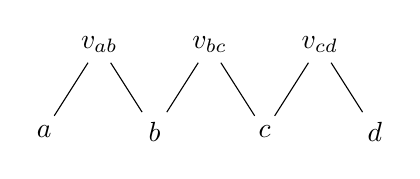
\begin{tikzpicture}[x=1.4cm,y=1.1cm]
\foreach \n/\x in {a/0,b/1,c/2,d/3} \node (\n) at (\x,0) {$\n$};
\node (vab) at (0.5,1) {$v_{ab}$};
\node (vbc) at (1.5,1) {$v_{bc}$};
\node (vcd) at (2.5,1) {$v_{cd}$};
\draw (a) -- (vab) -- (b) -- (vbc) -- (c) -- (vcd) -- (d);
\end{tikzpicture}
\end{center}

\begin{encadre}
\begin{contrexemple}[Énoncé de l'édition, page 68]
Dans ce modèle, $\leq$ est un ordre, $R$ est réflexive, symétrique et héritée vers le bas, chaque $\mathcal M_{\leq v}$ est formé d'éléments deux à deux compatibles et $\mathcal M$ est connexe, de sorte que la condition C\,4 est vide. Les parties saturées sont exactement
\[
\emptyset, \quad \{b\}, \quad \{c\}, \quad \{a, c\}, \quad \{b, d\}, \quad \mathcal M,
\]
et le treillis qu'elles forment n'est pas distributif : $\{b, d\} \wedge (\{b\} \vee \{c\}) = \{b, d\}$, tandis que $(\{b, d\} \wedge \{b\}) \vee (\{b, d\} \wedge \{c\}) = \{b\}$.
\end{contrexemple}
\end{encadre}

\begin{proof}
Deux éléments sont compatibles quand un même $\mathcal M_{\leq v}$ les contient ; ils sont disjoints quand de plus aucun élément n'est sous les deux. Les paires disjointes sont donc $\{a, b\}$, $\{b, c\}$ et $\{c, d\}$ : les trois $v$ ont un minorant commun avec chacun de leurs voisins, et $a$, $c$ par exemple ne sont pas compatibles. Le cosupport d'une partie est alors l'ensemble des voisins communs à tous ses éléments dans le chemin $a - b - c - d$, et le calcul des cent vingt-huit parties donne la liste annoncée : par exemple $\{b\}' = \{a, c\}$ et $\{a, c\}' = \{b\}$, $\{c\}' = \{b, d\}$ et $\{b, d\}' = \{c\}$, tandis que $\{b, c\}' = \emptyset$. Le support de $\{b\} \cup \{c\}$ est donc $\mathcal M$, et $\{b, d\} \cap \mathcal M = \{b, d\}$. De l'autre côté, $\{b, d\} \cap \{b\} = \{b\}$ et $\{b, d\} \cap \{c\} = \emptyset$, et le support de $\{b\}$ est $\{b\}$. En Lean, la liste des parties saturées et les deux calculs sont vérifiés par énumération exhaustive dans le noyau.
\end{proof}

\begin{remarque}
Le treillis obtenu est un hexagone : deux chaînes $\emptyset \subset \{b\} \subset \{b, d\} \subset \mathcal M$ et $\emptyset \subset \{c\} \subset \{a, c\} \subset \mathcal M$. La lecture notait que la distributivité tombe en général pour une relation symétrique quelconque ; elle tombe donc déjà sous les hypothèses que le dossier pose sur $(\mathcal M, \leq, R)$ jusqu'à la page~64. Le modèle ne code que cette structure ; les figures et les axiomes C\,1 à C\,3, qui portent sur elles, ne sont pas représentés.
\end{remarque}

Ne sont pas démontrés ici : que les axiomes de disjonction ultérieurs (C\,5 de la page~69, le \q{paquet d'axiomes de disjonction} de la page~85) rétablissent la distributivité ; le cas d'une relation $R$ toujours vraie, où les parties saturées sont les ouverts réguliers de $(\mathcal M, \leq)$ et forment une algèbre de Boole complète.
